\documentclass{article}

\usepackage{fancyhdr}
\usepackage{extramarks}
\usepackage{amsmath}
\usepackage{amssymb}
\usepackage{amsthm}
\usepackage{tikz}
\usepackage{enumerate}
\usepackage{listings}
\usepackage{algorithm}
\usepackage{algpseudocode}
\usepackage{caption}
\usepackage{xcolor}
\usepackage{subfig}
\usepackage{stmaryrd}
\usepackage{appendix}
\usepackage{multirow}

\usepackage[final]{nips_2017}

\usepackage[utf8]{inputenc} % allow utf-8 input
\usepackage[T1]{fontenc}    % use 8-bit T1 fonts
\usepackage{hyperref}       % hyperlinks
\usepackage{url}            % simple URL typesetting
\usepackage{booktabs}       % professional-quality tables
\usepackage{amsfonts}       % blackboard math symbols
\usepackage{nicefrac}       % compact symbols for 1/2, etc.
\usepackage{microtype}      % microtypography

\usepackage{longtable} % For tables that span multiple pages

\title{MGMT1317 Dynamic Programming HW4}

\author{Kangjie Xia\\
    ShanghaiTech University\\
    Shanghai, China \\
    \texttt{xiakj@shanghaitech.edu.cn} \\
    \And Weiming Luo\\
    ShanghaiTech University\\
    Shanghai, China \\
    \texttt{luowm@shanghaitech.edu.cn} \\
}


\newcommand{\E}{\mathrm{E}}

\begin{document}

\maketitle

\begin{abstract}
This report explores the application of a value iteration-based dynamic programming algorithm in the game of Monopoly. By modeling the game mechanics, state space, and action space, we developed various AI strategies and compared their performances through extensive simulations. Our research primarily focuses on four types of AI players: Random AI Player, Greedy AI Player, Basic AI Player, and Value Iteration AI Player. The results indicate that the Value Iteration AI Player performs best in long-term games, while Base AI Player excels in short-term games. Greedy AI Player performs optimally in medium-term games. The study demonstrates the effectiveness of the value iteration algorithm in optimizing game strategies and highlights potential areas for improvement, including enhanced state representation, hybrid AI strategies, and the incorporation of advanced reinforcement learning algorithms. Future work will focus on these areas to further enhance AI performance in various game scenarios.
\end{abstract}

\newpage

\section{Introduction}
Monopoly is a classic board game which simulates real estate trading and economic management, where players buy and sell properties, build houses and hotels, and collect rent to accumulate wealth. The ultimate goal is to bankrupt the opponents and be the last player standing at the top of the economic pyramid. 

\textcolor{red}{This paper explores the application of a value iteration-based dynamic programming algorithm to strategize the gameplay in Monopoly and compares this algorithm with random, greedy and basic AI algorithms, analyzing the results.}

    \subsection{Game Mechanics}    
    
    Main Components
    \begin{itemize}
        \item 
        Board: The board consists of a series of squares , each representing different properties, utilities(jail), or special events.
        \item 
        Balance: Balance represents cash used for buying properties, paying rent, and other transactions.
        \item 
        Property: Each property has its price and rent information.
        \item 
        Dice: Used to determine the number of spaces a player moves.
        \item 
        Chance and Community Chest Cards: Players draw these cards when landing on specific squares, following the instructions which can bring good or bad fortune.
    \end{itemize}
    
    Starting the Game
    \begin{itemize}
        \item 
        Each player selects a game token and places it on the starting square.
        \item 
        Players receive a set amount of money to start with.
        \item 
        The order of play is determined by rolling the dice.
    \end{itemize}

    Gameplay
    \begin{itemize}
        \item 
        Players take turns rolling the dice and moving their tokens according to the number rolled.
        \item 
        Depending on the square landed on, players can perform actions such as buying properties, paying rent, or drawing cards.
        \item 
        If a player lands on an unowned property, they can choose to buy it by paying the listed price.
        \item 
        If a player lands on a property owned by another player, they must pay rent to the owner.
        \item 
        In each game round, all players incur a fixed loss.
    \end{itemize}

    Winning the Game
    \begin{itemize}
        \item
        The goal is to accumulate wealth through buying and selling properties, and collecting rent. The game ends when all but one player have gone bankrupt, with the remaining player being declared the winner.
    \end{itemize}

\section{Model}
To model the Monopoly problem as a dynamic programming problem using a Markov chain, we first define the state and action spaces. For simplicity, we begin with the player and property spaces to construct the state space.

    \subsection{Player Space}
    The player space is used to characterize player information in the game. For a player, it is necessary to characterize all possible scenarios in a game through the player space. So the space should tell who it is, where it is and so on. And we can conclude the space as:
    
    $\{id, name, money, position, direction, jail\thinspace turns, alive, moveable, belief \footnotesize{\text{(Bayesian belief with a beta prior)}}\}$
    
    To clarify, let's make a simple explanation of some state variables. ''Jail turns'' helps to describe the state when a player enters jail, ''alive'' helps to judge when to end the game. And unlike single-player games, Monopoly is a multiplayer game where one's own decision-making should be based on anticipating the actions of others. So we use ''belief'' here to describe the anticipation of the actions of others.

    \subsection{Property Space}
    As for a property space, it is easy to understand that the space should characterize property information in the game. And the information of property is stable and we can conclude the space as:
    
    $\{location, name, details \footnotesize{\text{(price, rent, income, etc.)}}\}$
    
    \subsection{State Space}
    The state space needs to encompass all game information, ensuring that every possible game state corresponds to a unique element within the state space. From the player's perspective, there is the player currently required to perform an action and the player's information. From the property perspective, there is the property information. Additionally, it is necessary to include the linkage information of the board and the game round number. So we can conclude the space as:
    
    $\{current\thinspace player, player\thinspace info, property\thinspace info, map\thinspace connectivity, game\thinspace rounds\}$
    
    \subsection{Action Space}
    The action space, like the state space, is also very important. Since there are many actions a player can take in various game states, we can summarize and obtain the state space as follows:
    
    $\{no\thinspace action, buy\thinspace property, sell\thinspace property, pay\thinspace rent, get\thinspace reward, go\thinspace to\thinspace jail, stay\thinspace in\thinspace jail, move\}$

    However, although the total number of actions in the action space is large, in each game state, a player can either choose a single action or select one from two actions(buy property or sell property with no action), so the actual action space is not very large.
    
\section{AI Strategies}
We have designed a total of four AI algorithms to make decisions in the game of Monopoly, which are: Random AI Player, Greedy AI Player, Basic AI Player and Value Iteration AI Player. And the most important method, which uses a dynamic programming algorithm, is Value Iteration AI Player. Still we compared this algorithm with other AI algorithms and evaluated their effectiveness.

\subsection{Random AI Player}
The design approach for the random AI player is very simple: it randomly selects an action whenever a decision needs to be made. It is obvious that this behavior significantly differs from that of a human player and is far from the optimal choices. However, the random algorithm can effectively evaluate the lower bound of the Monopoly gameplay, making it a useful reference for comparison.

\subsection{Greedy AI Player}
The design approach for the greedy AI algorithm is to always choose ''buy property'' when faced with the choice between ''buy property'' and ''no action'', and to always choose ''no action'' when faced with the choice between ''sell property'' and ''no action''. This indicates that the player's greedy choices aim at maximizing the number of properties owned. Similar to the random AI algorithm, this behavior differs significantly from human decision-making and may also diverge from optimal strategies. However, as an extreme case algorithm, it serves well as a benchmark for comparison.

\subsection{Basic AI Player}
The Basic AI player attempts to replicate the thought process of a human player by estimating its expected survival rounds based on the current property ownership and financial status. Using this estimate, it compares the expected income from buying or selling properties versus taking no action, and makes decisions accordingly.

The calculation method for the expected survival rounds is as follows:
\begin{equation*}
    round = \frac{balance}{\frac{\sum other\_rent}{cell\_num}+reduce-\frac{\sum your\_rent}{cell\_num}(player\_num-1)}
\end{equation*}

Let's consider the decision-making process for buying a property as an example. The expected income from purchasing the property can be obtained using the following formula:
\begin{equation*}
    expecting\_gain = \frac{round\cdot (player\_num-1)}{cell\_num}+selling\_price\cdot \left(1-\left(\frac{cell\_num-1}{cell\_num}\right)^{round}\right)
\end{equation*}

And the expected loss from purchasing the property is equal to the price of the property.
\begin{equation*}
    expecting\_loss = buying\_price
\end{equation*}

So when $expecting\_gain$ is more than $expecting\_loss$, it chooses ''buy property''. Otherwise, it will choose ''no action''. The process for deciding whether to sell a property is similar to this. In summary, we have outlined the decision-making process of the Basic AI algorithm.

\subsection{Value Iteration AI Player}
\subsubsection{Value Iteration Algorithm}

The Value Iteration Algorithm is a method used in dynamic programming and reinforcement learning for computing the optimal policy and value function for a Markov Decision Process (MDP). The algorithm iteratively updates the value of each state until the values converge to the optimal value function. This optimal value function can then be used to derive the optimal policy for decision-making.

\textbf{Algorithm:}

The Value Iteration Algorithm consists of the following steps:

1. Initialize the value function \( V(s) \) for all states \( s \) arbitrarily, except that \( V(\text{terminal state}) = 0 \).

2. Repeat the following until convergence:
   \begin{itemize}
       \item For each state \( s \), update the value function using the Bellman equation:
       \[
       V(s) \leftarrow \max_a \sum_{s'} P(s' | s, a) [R(s, a, s') + \gamma V(s')]
       \]
       where:
       \begin{itemize}
           \item \( a \) is the action.
           \item \( s' \) is the next state.
           \item \( P(s' | s, a) \) is the transition probability from state \( s \) to state \( s' \) given action \( a \).
           \item \( R(s, a, s') \) is the reward received after transitioning from state \( s \) to state \( s' \) due to action \( a \).
           \item \( \gamma \) is the discount factor ( \( 0 \leq \gamma < 1 \) ).
       \end{itemize}
   \end{itemize}

3. The algorithm converges when the value function updates are smaller than a given threshold, i.e., \( \max_s | V_{\text{new}}(s) - V_{\text{old}}(s) | < \epsilon \).

4. Once the value function converges, derive the optimal policy \( \pi(s) \) as follows:
   \[
   \pi(s) = \arg\max_a \sum_{s'} P(s' | s, a) [R(s, a, s') + \gamma V(s')]
   \]

\textbf{Pseudocode:}

\begin{algorithm}
\caption{Value Iteration Algorithm}
    \begin{algorithmic}[1]
        \Procedure{ValueIteration}{$States, Actions, P, R, \gamma, \epsilon$}
            \For{each state $s$} \Comment{Initialize value function}
                \State $V(s) \gets$ arbitrary value (except $V(\text{terminal state}) \gets 0$)
            \EndFor
            \Repeat
                \State $\Delta \gets 0$
                \For{each state $s$}
                    \State $v \gets V(s)$
                    \State $V(s) \gets \max\limits_a \sum\limits_{s'} P(s' | s, a) [R(s, a, s') + \gamma V(s')]$
                    \State $\Delta \gets \max(\Delta, |v - V(s)|)$
                \EndFor
            \Until{$\Delta < \epsilon$}
            \For{each state $s$} \Comment{Derive the optimal policy}
                \State $\pi(s) \gets \arg\max\limits_a \sum\limits_{s'} P(s' | s, a) [R(s, a, s') + \gamma V(s')]$
            \EndFor
        \EndProcedure
    \end{algorithmic}
\end{algorithm}

\subsubsection{Basic Idea}
    The core idea is to simplify the state by ignoring position information and focusing on the financial relationship.
    
    The simplified states are pre-calculated for all corresponding actions. The state values are updated using the previous value until convergence or a maximum number of iterations is reached. The trained state data is saved and can be reloaded for multiple training sessions. After creation, the actions are predicted based on the maximum value of $V(s') + r(a)$.

\subsubsection{Simplified Game States}
    Since the complexity of each iteration of the value iteration algorithm is \( |S|^2|A| \), we need to simplify the size of the state space in order to converge within a limited time. The size of the action space does not exceed 2, so we only need to simplify the size of the game state space.
    
    A significant portion of the state space is occupied by the positions of the players and the locations of the buildings on the map. Therefore, simplifying the positional information is essential. One straightforward idea is that, since the player's movement each step involves a random factor, we can attempt to ignore the player's position and only count the number of key buildings on the map to achieve a reduction in the total number of game states.
    
    Meanwhile, since the financial information of the players has an infinite space (any integer), we must discretize it. Other information is mostly extremely limited (e.g., whether the player is alive, jail turns) or insignificant (player ID, name), so we can directly inherit it.
    
    Then, each simplified game state is encoded such that each game state corresponds to a unique string and is stored in a dictionary-type variable where the key is the string, and the value is also a dictionary variable. In this dictionary, the key is the player's ID, and the value is the value of this game state for that player. For a specific player's game state value, it is the player's value in the dictionary (where the state string is the key) minus the opponent's value.
    
    \begin{enumerate}
        \item 
        \textbf{Simplifying the player state}
    
            We have transformed the discrete financial data into a fixed set of financial states, where it's defined as following:
            \begin{itemize}
                \item 'safe': money $>$ 1000
                \item 'risky\textasciitilde': money $<$ 1000, $\Delta <$ 200, rate $\in$ [0.75, 1.33]
                \item 'risky\textgreater': money higher than opponent
                \item 'risky\textless': money lower than opponent
            \end{itemize}
            
            In addition, we also retain information about the player's jail turns and whether they are alive.
            i.e.
    
            \[
                SPS = \{ (b, j, a) \}
            \]
    
            where \( SPS \) means the simplified players' state, \( b, j, a \) refer to balance state, jail turns and alive.
        
        \item
        \textbf{Simplifying the map state}
            
            Since most plots are immutable, we only need to encode the plots that may change for each state, namely the building types. Since we have omitted the positional information, we only need to count the number of buildings of different ownership.
            i.e.
    
            \[
                SMS = \{ (N_1, N_2, N_e) \}
            \]
    
            where \( SMS \) means the simplified map state, \( N_1 \) refers to the number of buildings belong to player 1, \( N_1 \) refers to the ones belong to player 2, \( N_e \) refers to the number of empty buildings.
    \end{enumerate}
    
    In summary, the Simplified Game State includes the Simplified Player States of two players and the Simplified Map State.
    i.e.
    
    \[
        SGS = \{ (b_1, j_1, a_1, b_2, j_2, a_2, N_1, N_2, N_e) \}
    \]

\subsubsection{Get Next Game State}
    Since we have already ignored the location information, we assume that each step by the player lands randomly at any position on the map. Based on the state's SMS and the global map information, we can determine the probability distribution of the player landing in different areas, which is to obtain the probability distribution for different action lists. Then, all we need to do is to iterate through each action in every action list, calculate the next game state, and obtain the corresponding SGS, and look up the value associated with that SGS, taking the action associated with the highest value among all values as the optimal action in that action list. Finally, by multiplying by the probability of that action list and summing up for all action lists, we can obtain the desired outcome.


\subsubsection{Implementation Details}
    Even if we can obtain a converged game state value within a limited time, another problem arises: due to the simplification of the financial relationship, during state transition, we often encounter a situation where a player's funds decrease when buying or selling a piece of land, but the balance state does not change. This is equivalent to buying or selling a piece of land for nothing. Therefore, we need to find a most typical game state corresponding to this state before simplification, and this state will continuously change with the cycle.
    
    To solve this problem, we need to introduce specific balance values, and then set a weight for this state. During training, we need to modify the original state according to the new state, where the weight of SGS will increase progressively, while the included SPS and SMS will be weighted and averaged with the new state until it converges to a fixed value.


\section{Simulation Results}
\subsection{Game Interface}
\begin{figure}[H]
    \centering
         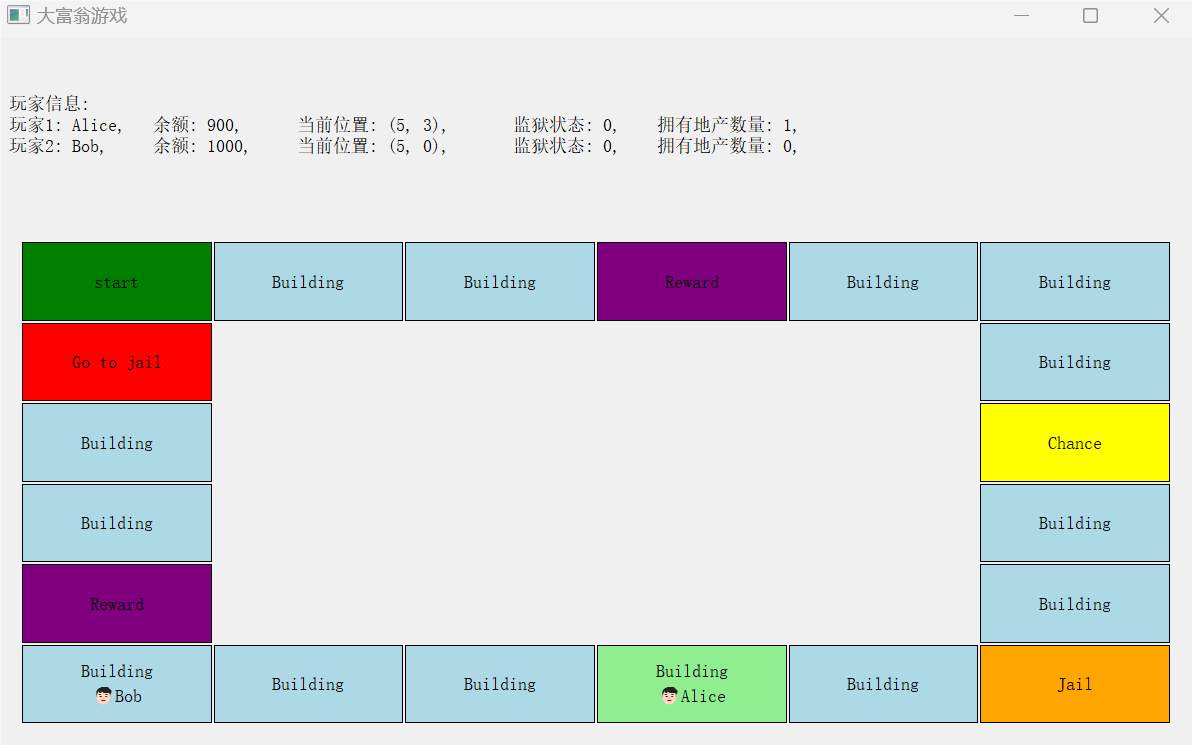
\includegraphics[width=\linewidth]{figures/Game_Interface1.png}
         \caption{Game Interface Example1}
         \label{fig:Game_Interface1}
\end{figure}

\begin{figure}[H]
    \centering
         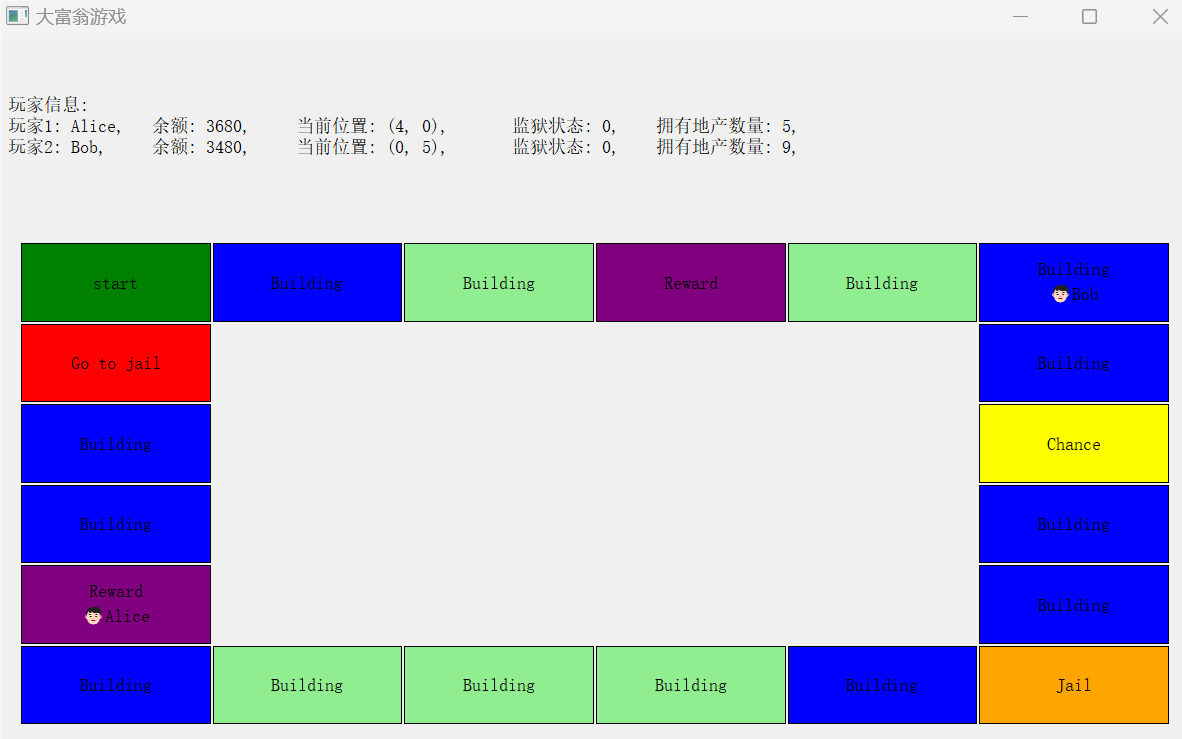
\includegraphics[width=\linewidth]{figures/Game_Interface2.png}
         \caption{Game Interface Example2}
         \label{fig:Game_Interface2}
\end{figure}

\subsection{Player Configurations}
    \subsubsection{Global Constants}
    \begin{align*}
        \text{seed} &= MGMT1317 \\
        \text{round reduce} &= 20 \\
        \text{selling rate} &= 0.5 \\
        \gamma &= 0.99 \\
    \end{align*}

    where seed is the random seed, round reduce is the number which each player's balance will reduce each round, selling rate is the rate that players sell buildings, and \( \gamma \) is the discount rate during training the ValueIterationPlayer.

    \subsubsection{Comparison Results}
    \begin{longtable}{|p{3cm}|p{1cm}|p{1.3cm}|p{2.5cm}|p{1cm}|p{1.3cm}|p{1.2cm}|}
        \hline
        \textbf{Player 1} & \textbf{Win Rate 1} & \textbf{Avg Round 1} & \textbf{Player 2} & \textbf{Win Rate 2} & \textbf{Avg Round 2} & \textbf{Start\,\,\,\, Balance}\\
        \hline
        \endfirsthead
        
        \multicolumn{7}{c}%
        {{\bfseries \tablename\ \thetable{} -- continued from previous page}} \\
        \hline
        \textbf{Player 1} & \textbf{Win Rate 1} & \textbf{Avg Round 1} & \textbf{Player 2} & \textbf{Win Rate 2} & \textbf{Avg Round 2} & \textbf{Start\,\,\, Balance}\\
        \hline
        \endhead
        
        \hline \multicolumn{7}{|r|}{{Continued on next page}} \\ \hline
        \endfoot
        
        \hline
        \caption{Game Performance Analysis}\\
        \endlastfoot

        % ValueIterationPlayer
        \multirow{9}{*}{ValueIterationPlayer} & 100\% & 233.346 & \multirow{3}{*}{RandomPlayer} & 0.0\% & NA  & 5000 \\
        \cline{2-3} \cline{5-7}
        & 89.1\% & 96.897 &  & 10.9\% & 91.174 & 2000 \\
        \cline{2-3} \cline{5-7}
        & 18.0\% & 35.339 &  & 82.0\% & 25.366 & 1000 \\
        \cline{2-7}
        & 56.6\% & 349.472 & \multirow{3}{*}{BaseAIPlayer} & 43.4\% & 357.023 & 5000 \\
        \cline{2-3} \cline{5-7}
        & 62.4\% & 100.958 &  & 37.6\% & 92.293 & 2000 \\
        \cline{2-3} \cline{5-7}
        & 4.9\% & 49.612 &  & 95.1\% & 26.186 & 1000 \\
        \cline{2-7}
        & 52.6\% & 354.949 & \multirow{3}{*}{GreedyAIPlayer} & 47.4\% & 362.660 & 5000 \\
        \cline{2-3} \cline{5-7}
        & 46.0\% & 105.513 &  & 54.0\% & 108.083 & 2000 \\
        \cline{2-3} \cline{5-7}
        & 50.2\% & 26.026 &  & 49.8\% & 26.406 & 1000 \\
        \hline
        % BaseAIPlayer
        \multirow{6}{*}{BaseAIPlayer} & 100.0\% & 234.072 & \multirow{3}{*}{RandomPlayer} & 0.0\% & NA & 5000 \\
        \cline{2-3} \cline{5-7}
        & 92.6\% & 95.069 &  & 7.4\% & 105.703 & 2000 \\
        \cline{2-3} \cline{5-7}
        & 90.3\% & 40.626 &  & 9.7\% & 57.031 & 1000 \\
        \cline{2-7}
        & 49.3\% & 349.458 & \multirow{3}{*}{GreedyAIPlayer} & 50.7\% & 353.458 & 5000 \\
        \cline{2-3} \cline{5-7}
        & 38.8\% & 90.588 &  & 61.2\% & 99.538 & 2000 \\
        \cline{2-3} \cline{5-7}
        & 96.4\% & 24.186 &  & 3.6\% & 49.0 & 1000 \\
        \hline
        % GreedyAIPlayer
        \multirow{3}{*}{GreedyAIPlayer} & 100.0\% & 234.072 & \multirow{3}{*}{RandomPlayer} & 0.0\% & NA & 5000 \\
        \cline{2-3} \cline{5-7}
        & 94.1\% & 96.566 &  & 5.9\% & 88.864 & 2000 \\
        \cline{2-3} \cline{5-7}
        & 18.1\% & 33.530 &  & 81.9\% & 24.943 & 1000 \\

    \end{longtable}

    After fixing the random seed and game parameters, and comparing different strategy AIs over 1000 games in long, medium, and short game lengths respectively, we found:

    In long-term games, the ValueIterationPlayer performs best, followed by BaseAIPlayer and GreedyAIPlayer, while RandomPlayer performs the worst (with no victories).
    
    In medium-term games, GreedyAIPlayer performs the best, with ValueIterationPlayer slightly behind, followed by BaseAIPlayer, and RandomPlayer still at the bottom.
    
    In short-term games, BaseAIPlayer performs the best, followed by RandomPlayer, with ValueIterationPlayer and GreedyAIPlayer performing the worst.

    \subsubsection{Comparison Conclusion}
    Based on the win rate data and combined with the UI display process, we find:
    \begin{enumerate}
        \item The behavior of \textit{RandomPlayer} has no discernible pattern.
        \item \textit{GreedyAIPlayer} only engages in purchasing activities and performs poorly in the short term, exhibiting an extremely aggressive overall behavior.
        \item \textit{ValueIterationPlayer} tends to purchase territories at the onset of the game but has a low inclination to sell, choosing to do so only when close to failure. This strategy results in it being the most successful entity in medium to long-term games, with a generally aggressive performance.
        \item \textit{BaseAIPlayer} purchases territories at the start of medium to long-term games but shows a high propensity to sell early to ensure survival, making it the most effective strategy in short-term games with a more conservative overall performance.
    \end{enumerate}
    
\section{Improvement}
In the future, if there is an opportunity, we plan to implement the following contents:
\begin{enumerate}
    \item \textbf{Strategy Iteration}:
    Strategy iteration is an iterative method used in dynamic programming and reinforcement learning to improve the decision-making policy. By alternating between policy evaluation and policy improvement steps, we can systematically enhance the AI's strategy. This method is particularly useful for optimizing actions in complex decision environments. The process involves:
    \begin{itemize}
        \item \textit{Policy Evaluation}: Calculating the value of a given policy by determining the expected returns from following that policy.
        \item \textit{Policy Improvement}: Updating the policy based on the evaluation to choose better actions.
        \item \textit{Iterative Refinement}: Repeating the evaluation and improvement steps until the policy converges to an optimal strategy.
    \end{itemize}

    \item \textbf{Decision Tree Algorithms}:
    Decision tree algorithms can be employed to enhance the decision-making process in the game. By constructing a tree-based model, we can systematically evaluate the potential outcomes of different actions at each stage of the game. This approach allows for a more structured and interpretable decision-making process, making it easier to analyze and optimize strategies. Specifically, we can use techniques such as:
    \begin{itemize}
        \item \textit{Classification and Regression Trees (CART)}: To predict the optimal actions based on the current state of the game.
        \item \textit{Random Forests}: To create an ensemble of decision trees that reduce overfitting and improve generalization to new game scenarios.
        \item \textit{Gradient Boosting Trees}: To iteratively refine decisions by focusing on errors made in previous iterations, thereby improving overall strategy performance.
    \end{itemize}

    \item \textbf{Incorporating Reinforcement Learning Algorithms}:
   Implementing more advanced reinforcement learning algorithms such as Deep Q-Networks (DQN), Proximal Policy Optimization (PPO), or Actor-Critic methods could potentially improve the AI's performance by allowing it to learn more complex strategies and adapt to different game scenarios dynamically.

    \item \textbf{Enhanced State Representation}:
   Improving the state representation by including more detailed information about the game. For instance, incorporating historical data of player actions, more granular financial data, and other contextual information that could help in making more informed decisions.

    \item \textbf{Hybrid AI Strategies}:
   Combining different AI strategies to create a hybrid model that can switch between strategies based on the game context. For example, using a greedy approach in early stages and switching to a more conservative or value iteration-based approach in later stages.
\end{enumerate}
   
\section{Conclusion}
We explored the application of a value iteration-based dynamic programming algorithm in the game of Monopoly. By modeling the game mechanics, state space, and action space, we developed various AI strategies and compared their performances through extensive simulations. The value iteration-based dynamic programming algorithm provides a robust strategy for playing Monopoly. 

Our results indicated that:
\begin{itemize}
    \item \textbf{In long-term games}, the ValueIterationPlayer performed the best, followed by BaseAIPlayer and GreedyAIPlayer, while RandomPlayer performed the worst (with no victories).
    \item \textbf{In medium-term games}, GreedyAIPlayer performed the best, with ValueIterationPlayer slightly behind, followed by BaseAIPlayer, and RandomPlayer still at the bottom.
    \item \textbf{In short-term games}, BaseAIPlayer performed the best, followed by RandomPlayer, with ValueIterationPlayer and GreedyAIPlayer performing the worst.
\end{itemize}

Our study demonstrated the effectiveness of the value iteration algorithm in optimizing game strategies and highlighted the potential for further improvements. Future work will focus on incorporating more advanced algorithms and refining the state and action representations to enhance AI performance in various game scenarios.

\end{document}